% RingKernel Executive Overview
% Compile with: pdflatex ringkernel-executive-overview.tex (run twice for TOC)
\documentclass[11pt,a4paper]{article}

% ── Packages ──────────────────────────────────────────────────────────────────
\usepackage[utf8]{inputenc}
\usepackage[T1]{fontenc}
\usepackage{lmodern}
\usepackage[margin=2.4cm]{geometry}
\usepackage{graphicx}
\usepackage{xcolor}
\usepackage{titlesec}
\usepackage{enumitem}
\usepackage{booktabs}
\usepackage{tabularx}
\usepackage{multirow}
\usepackage{fancyhdr}
\usepackage{hyperref}
\usepackage{amssymb}
\usepackage{tcolorbox}
\usepackage{tikz}
\usepackage{pgfplots}
\pgfplotsset{compat=1.18}
\usetikzlibrary{arrows.meta, positioning, calc, shapes.geometric, backgrounds, fit}

% ── Colours ───────────────────────────────────────────────────────────────────
\definecolor{brand}{HTML}{1B2D45}      % Deep navy
\definecolor{accent}{HTML}{E85D04}     % Burnt orange (GPU warmth)
\definecolor{highlight}{HTML}{0096C7}  % Bright cyan
\definecolor{success}{HTML}{2D936C}    % Green
\definecolor{lightbg}{HTML}{F4F6F9}    % Light background
\definecolor{midgray}{HTML}{6C757D}    % Muted text

% ── Heading styles ────────────────────────────────────────────────────────────
\titleformat{\section}
  {\Large\bfseries\color{brand}}
  {\thesection}{1em}{}[\vspace{-0.4em}\textcolor{accent}{\rule{\textwidth}{1.2pt}}]

\titleformat{\subsection}
  {\large\bfseries\color{brand}}
  {\thesubsection}{0.8em}{}

\titleformat{\subsubsection}
  {\normalsize\bfseries\color{accent}}
  {\thesubsubsection}{0.6em}{}

% ── Header / Footer ──────────────────────────────────────────────────────────
\pagestyle{fancy}
\fancyhf{}
\renewcommand{\headrulewidth}{0.4pt}
\fancyhead[L]{\small\textcolor{midgray}{RingKernel --- Executive Overview}}
\fancyhead[R]{\small\textcolor{midgray}{v0.4.0}}
\fancyfoot[C]{\small\textcolor{midgray}{\thepage}}

% ── Custom boxes ──────────────────────────────────────────────────────────────
\tcbset{
  keybox/.style={
    colback=lightbg, colframe=accent, boxrule=0.6pt,
    arc=3pt, left=8pt, right=8pt, top=6pt, bottom=6pt,
    fonttitle=\bfseries\color{brand}, title=#1
  },
  statbox/.style={
    colback=white, colframe=brand, boxrule=0.8pt,
    arc=4pt, left=6pt, right=6pt, top=4pt, bottom=4pt,
    width=0.30\textwidth
  }
}

% ── Hyperref setup ────────────────────────────────────────────────────────────
\hypersetup{
  colorlinks=true,
  linkcolor=brand,
  urlcolor=highlight,
  citecolor=brand,
  pdftitle={RingKernel -- GPU-Native Persistent Actor Model},
  pdfauthor={Michael Ivertowski},
  pdfsubject={Executive Overview},
}

% ══════════════════════════════════════════════════════════════════════════════
\begin{document}

% ── Title page ────────────────────────────────────────────────────────────────
\begin{titlepage}
\begin{tikzpicture}[remember picture, overlay]
  % Background gradient bar
  \fill[brand] (current page.north west) rectangle
    ([yshift=-9cm]current page.north east);
  % Accent stripe
  \fill[accent] ([yshift=-9cm]current page.north west) rectangle
    ([yshift=-9.4cm]current page.north east);
  % Decorative dots
  \foreach \x in {0.5,1.0,...,5.0} {
    \foreach \y in {0.5,1.0,...,3.0} {
      \fill[white, opacity=0.04] ([xshift=\x cm, yshift=-\y cm]current page.north west)
        circle (1.5pt);
    }
  }
\end{tikzpicture}

\vspace*{1.5cm}
\begin{flushleft}
  {\fontsize{38}{44}\selectfont\bfseries\textcolor{white}{RingKernel}}\\[0.5em]
  {\fontsize{16}{20}\selectfont\textcolor{white!85}{GPU-Native Persistent Actor Model for Rust}}\\[0.3em]
  {\large\textcolor{white!65}{Lock-Free Message Passing \textbullet{} Hybrid Logical Clocks \textbullet{} Multi-Backend}}\\[0.3em]
  {\normalsize\textcolor{white!50}{Rust core \textbullet{} Python wrapper \textbullet{} CUDA \textbullet{} WebGPU \textbullet{} Metal \textbullet{} CPU}}
\end{flushleft}

\vspace{5.5cm}

\begin{flushleft}
  \textcolor{midgray}{\large Executive Overview}\\[0.8em]
  {\Large\textcolor{brand}{\textbf{Version 0.4.0}}}\\[1.5em]
  \textcolor{midgray}{%
    A framework for treating GPU compute units as persistent actors\\
    with causal ordering, zero-copy messaging, and enterprise-grade tooling.%
  }
\end{flushleft}

\vfill
\begin{flushleft}
  \textcolor{midgray}{\small
    Built with Rust \& Python \textbullet{} 20+ modular crates \textbullet{} 950+ tests\\[4pt]
    Open-source (Apache-2.0) \textbullet{} Published on crates.io \& PyPI\\[4pt]
    \textbf{Contact:} \href{mailto:michael.ivertowski@ch.ey.com}{michael.ivertowski@ch.ey.com}
  }
\end{flushleft}
\end{titlepage}

% ── Table of Contents ─────────────────────────────────────────────────────────
\tableofcontents
\newpage

% ══════════════════════════════════════════════════════════════════════════════
\section{Executive Summary}

RingKernel is a GPU-native persistent actor model framework for Rust. It
enables GPU-accelerated actor systems where compute kernels persist for the
lifetime of a simulation, exchanging messages through lock-free ring buffers
and maintaining causal ordering via hybrid logical clocks (HLC). Written
entirely in Rust for memory safety and performance, RingKernel provides a
unified programming model across CUDA, WebGPU, Metal, and CPU backends.

\begin{tcolorbox}[keybox={Why RingKernel?}]
\begin{itemize}[leftmargin=1.2em, itemsep=3pt]
  \item \textbf{Persistent GPU actors} --- kernels remain resident on the GPU,
        eliminating per-command launch overhead (11,327$\times$ faster command
        injection vs.\ traditional kernel dispatch).
  \item \textbf{Zero-copy message passing} --- rkyv-based serialization enables
        host$\leftrightarrow$GPU and kernel-to-kernel (K2K) communication without
        intermediate copies.
  \item \textbf{Causal ordering} --- hybrid logical clocks provide happened-before
        semantics across heterogeneous compute units.
  \item \textbf{Multi-backend} --- write once, run on CUDA, WebGPU, Metal, or CPU.
        Rust DSL transpilers generate native GPU code (CUDA~C, WGSL).
  \item \textbf{Enterprise-ready} --- built-in observability, circuit breakers,
        multi-GPU coordination, TLS, RBAC, and rate limiting.
\end{itemize}
\end{tcolorbox}

\subsection{At a Glance}

\vspace{0.6em}
\begin{center}
\begin{tabular}{@{}c@{\hspace{1.8em}}c@{\hspace{1.8em}}c@{}}
% Row 1
\begin{tcolorbox}[statbox, width=4.8cm]
  \centering
  {\fontsize{26}{30}\selectfont\bfseries\textcolor{accent}{93B}}\\[3pt]
  {\small elem/sec CUDA throughput}
\end{tcolorbox} &
\begin{tcolorbox}[statbox, width=4.8cm]
  \centering
  {\fontsize{26}{30}\selectfont\bfseries\textcolor{accent}{11,327$\times$}}\\[3pt]
  {\small faster command injection}
\end{tcolorbox} &
\begin{tcolorbox}[statbox, width=4.8cm]
  \centering
  {\fontsize{26}{30}\selectfont\bfseries\textcolor{accent}{280$\times$}}\\[3pt]
  {\small GPU stencil speedup}
\end{tcolorbox} \\[0.8em]
% Row 2
\begin{tcolorbox}[statbox, width=4.8cm]
  \centering
  {\fontsize{26}{30}\selectfont\bfseries\textcolor{accent}{20+}}\\[3pt]
  {\small modular Rust crates}
\end{tcolorbox} &
\begin{tcolorbox}[statbox, width=4.8cm]
  \centering
  {\fontsize{26}{30}\selectfont\bfseries\textcolor{accent}{950+}}\\[3pt]
  {\small unit \& integration tests}
\end{tcolorbox} &
\begin{tcolorbox}[statbox, width=4.8cm]
  \centering
  {\fontsize{26}{30}\selectfont\bfseries\textcolor{accent}{4}}\\[3pt]
  {\small GPU backends}
\end{tcolorbox}
\end{tabular}
\end{center}

% ══════════════════════════════════════════════════════════════════════════════
\newpage
\section{Core Abstractions}

\subsection{Persistent Actor Model}

Traditional GPU programming launches kernels, waits for results, and repeats.
RingKernel keeps actors \emph{resident} on the GPU, processing messages in a
persistent loop. This eliminates kernel launch overhead and enables real-time
interactive workloads.

\begin{table}[h!]
\centering
\renewcommand{\arraystretch}{1.25}
\begin{tabularx}{\textwidth}{>{\bfseries\color{brand}}l X}
\toprule
\textbf{Abstraction} & \textbf{Description} \\
\midrule
RingMessage &
  Trait for GPU-transferable messages using rkyv zero-copy serialization with
  automatic type ID generation and correlation tracking. \\
MessageQueue &
  Lock-free ring buffer (power-of-2 capacity) for host$\leftrightarrow$GPU and
  kernel-to-kernel message passing with atomic head/tail pointers. \\
ControlBlock &
  128-byte GPU-resident structure managing kernel lifecycle state, activation,
  and termination signals. \\
HlcTimestamp &
  Hybrid logical clock combining physical time with logical counters for
  causal ordering across heterogeneous compute units. \\
K2K Broker &
  Kernel-to-kernel direct messaging broker with endpoint registration and
  topic-based publish/subscribe with wildcard matching. \\
RingContext &
  GPU intrinsics facade passed to kernel handlers, providing thread indexing,
  synchronization, shared memory, and warp operations. \\
\bottomrule
\end{tabularx}
\end{table}

\subsection{Message Flow}

\begin{center}
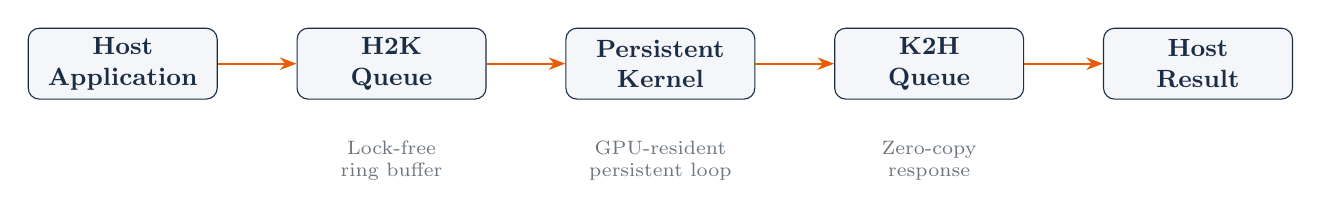
\begin{tikzpicture}[
  node distance=1.0cm,
  box/.style={draw=brand, fill=lightbg, rounded corners=4pt,
              minimum width=2.4cm, minimum height=0.9cm,
              font=\small\bfseries, text=brand, align=center},
  arr/.style={-{Stealth[length=6pt]}, thick, color=accent}
]
  \node[box] (host) {Host\\Application};
  \node[box, right=of host] (h2k) {H2K\\Queue};
  \node[box, right=of h2k] (kernel) {Persistent\\Kernel};
  \node[box, right=of kernel] (k2h) {K2H\\Queue};
  \node[box, right=of k2h] (result) {Host\\Result};

  \draw[arr] (host) -- (h2k);
  \draw[arr] (h2k) -- (kernel);
  \draw[arr] (kernel) -- (k2h);
  \draw[arr] (k2h) -- (result);

  \node[below=0.4cm of h2k, font=\scriptsize\color{midgray}, align=center]
    {Lock-free\\ring buffer};
  \node[below=0.4cm of kernel, font=\scriptsize\color{midgray}, align=center]
    {GPU-resident\\persistent loop};
  \node[below=0.4cm of k2h, font=\scriptsize\color{midgray}, align=center]
    {Zero-copy\\response};
\end{tikzpicture}
\end{center}

% ══════════════════════════════════════════════════════════════════════════════
\newpage
\section{GPU Backends \& Code Generation}

\subsection{Multi-Backend Architecture}

RingKernel supports four backends through the \texttt{RingKernelRuntime} trait.
Selection is automatic or explicit via feature flags:

\begin{table}[h!]
\centering
\renewcommand{\arraystretch}{1.2}
\begin{tabularx}{\textwidth}{>{\bfseries\color{brand}}l l X}
\toprule
\textbf{Backend} & \textbf{Feature} & \textbf{Capabilities} \\
\midrule
CUDA &
  \texttt{cuda} &
  Full persistent actors, cooperative groups, multi-stream execution,
  PTX caching, GPU memory pool, NVTX profiling. \\
WebGPU &
  \texttt{wgpu} &
  Cross-platform (Vulkan, Metal, DX12), host-driven dispatch loop,
  compute shader generation via WGSL transpiler. \\
Metal &
  \texttt{metal} &
  macOS/iOS scaffold with runtime, buffer management, and pipeline
  infrastructure. \\
CPU &
  \texttt{cpu} &
  Always available. Tokio-based async runtime for testing, development,
  and fallback execution. \\
\bottomrule
\end{tabularx}
\end{table}

\subsection{Rust-to-GPU Transpilers}

Write GPU kernels in a Rust DSL and transpile to native GPU code. The
transpilers support four kernel types:

\begin{table}[h!]
\centering
\renewcommand{\arraystretch}{1.2}
\begin{tabularx}{\textwidth}{>{\bfseries\color{brand}}l l X}
\toprule
\textbf{Kernel Type} & \textbf{Targets} & \textbf{Description} \\
\midrule
Global Kernels &
  CUDA, WGSL &
  Generic GPU compute (SAXPY, reductions, transforms). \\
Stencil Kernels &
  CUDA, WGSL &
  Grid-based operations with \texttt{GridPos} abstraction for 2D/3D
  neighbor access, shared memory tiling, and halo exchange. \\
Ring Kernels &
  CUDA &
  Persistent actor kernels with envelope-based messaging, HLC clocks,
  K2K routing, and ControlBlock lifecycle management. \\
Persistent FDTD &
  CUDA &
  Truly persistent 3D simulation kernels with cooperative groups,
  H2K/K2H queues, and tile-based halo exchange. \\
\bottomrule
\end{tabularx}
\end{table}

\noindent
The DSL provides 120+ GPU intrinsics across 13 categories (synchronization,
atomics, math, trigonometry, warp operations, shared memory, and more).
The \texttt{ringkernel-ir} crate provides a unified intermediate
representation that lowers to CUDA, WGSL, or MSL.

% ══════════════════════════════════════════════════════════════════════════════
\newpage
\section{Performance}

\subsection{Throughput Benchmarks (RTX Ada)}

\begin{table}[h!]
\centering
\renewcommand{\arraystretch}{1.2}
\begin{tabularx}{\textwidth}{>{\bfseries\color{brand}}l r r r}
\toprule
\textbf{Benchmark} & \textbf{Throughput} & \textbf{Batch Time} & \textbf{vs.\ CPU} \\
\midrule
CUDA Codegen (1M floats) & 93B elem/sec & 0.5\,$\mu$s & 12,378$\times$ \\
CUDA SAXPY PTX           & 77B elem/sec & 0.6\,$\mu$s & 10,258$\times$ \\
GPU Stencil (64\textsuperscript{3}) & 78,046 Mcells/s & --- & 280.6$\times$ \\
GPU Persistent           & 18.2 Mcells/s & --- & 1.2$\times$ \\
CPU Baseline (Rayon)     & 278 Mcells/s  & --- & 1.0$\times$ \\
\bottomrule
\end{tabularx}
\end{table}

\subsection{Persistent vs.\ Traditional Kernels}

The persistent actor model excels at \textbf{interactive command latency}:

\begin{table}[h!]
\centering
\renewcommand{\arraystretch}{1.2}
\begin{tabularx}{\textwidth}{>{\bfseries\color{brand}}l r r l}
\toprule
\textbf{Operation} & \textbf{Traditional} & \textbf{Persistent} & \textbf{Winner} \\
\midrule
Inject (send command) & 317\,$\mu$s & 0.03\,$\mu$s & \textcolor{success}{\textbf{Persistent 11,327$\times$}} \\
Query (read state)    & 0.01\,$\mu$s & 0.01\,$\mu$s & Tie \\
Single step (compute) & 3.2\,$\mu$s  & 163\,$\mu$s  & Traditional 51$\times$ \\
Mixed workload        & 40.5\,ms    & 15.3\,ms    & \textcolor{success}{\textbf{Persistent 2.7$\times$}} \\
\bottomrule
\end{tabularx}
\end{table}

\begin{tcolorbox}[keybox={When to Use Each Approach}]
\begin{itemize}[leftmargin=1.2em, itemsep=3pt]
  \item \textbf{Batch compute} (1000s of steps) --- Traditional kernels for
        maximum per-step throughput.
  \item \textbf{Interactive commands} --- Persistent actors for 11,327$\times$
        faster command injection via mapped memory.
  \item \textbf{Real-time GUI} (60\,FPS) --- Persistent actors deliver 2.7$\times$
        more operations per 16\,ms frame budget.
  \item \textbf{Dynamic topology} --- Persistent actors avoid kernel relaunch
        when the actor graph changes.
\end{itemize}
\end{tcolorbox}

% ══════════════════════════════════════════════════════════════════════════════
\newpage
\section{Architecture}

\subsection{Layered Crate Architecture}

\begin{center}
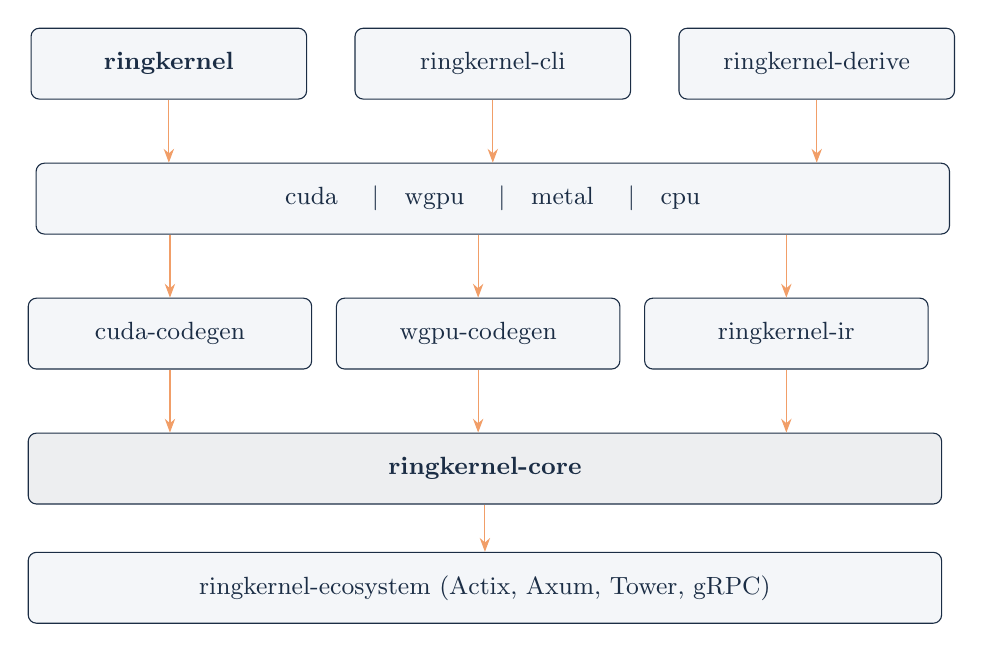
\begin{tikzpicture}[
  node distance=0.5cm,
  layer/.style={draw=brand, fill=lightbg, rounded corners=3pt,
                minimum height=0.9cm, font=\small, text=brand, align=center},
  arr/.style={-{Stealth[length=5pt]}, color=accent!60}
]
  % Top layer
  \node[layer, minimum width=3.5cm] (facade) {\textbf{ringkernel}};
  \node[layer, minimum width=3.5cm, right=0.6cm of facade] (cli) {ringkernel-cli};
  \node[layer, minimum width=3.5cm, right=0.6cm of cli] (derive) {ringkernel-derive};

  % Backend layer
  \node[layer, minimum width=11.6cm, below=0.8cm of cli] (backends)
    {cuda \quad\textbar\quad wgpu \quad\textbar\quad metal \quad\textbar\quad cpu};

  % Codegen layer
  \node[layer, minimum width=3.6cm, below=0.8cm of backends.south west,
        anchor=north west, xshift=-0.1cm] (cudacg) {cuda-codegen};
  \node[layer, minimum width=3.6cm, right=0.3cm of cudacg] (wgpucg) {wgpu-codegen};
  \node[layer, minimum width=3.6cm, right=0.3cm of wgpucg] (ir) {ringkernel-ir};

  % Core
  \node[layer, minimum width=11.6cm, below=0.8cm of cudacg.south west,
        anchor=north west, fill=brand!8]
    (core) {\textbf{ringkernel-core}};

  % Ecosystem
  \node[layer, minimum width=11.6cm, below=0.6cm of core]
    (eco) {ringkernel-ecosystem (Actix, Axum, Tower, gRPC)};

  % Arrows
  \draw[arr] (facade.south) -- (facade.south |- backends.north);
  \draw[arr] (cli.south) -- (backends.north);
  \draw[arr] (derive.south) -- (derive.south |- backends.north);

  \draw[arr] (backends.south -| cudacg) -- (cudacg.north);
  \draw[arr] (backends.south -| wgpucg) -- (wgpucg.north);
  \draw[arr] (backends.south -| ir) -- (ir.north);

  \draw[arr] (cudacg.south) -- (cudacg.south |- core.north);
  \draw[arr] (wgpucg.south) -- (wgpucg.south |- core.north);
  \draw[arr] (ir.south) -- (ir.south |- core.north);
  \draw[arr] (core.south) -- (eco.north);
\end{tikzpicture}
\end{center}

\subsection{Enterprise Infrastructure}

\begin{table}[h!]
\centering
\renewcommand{\arraystretch}{1.2}
\begin{tabularx}{\textwidth}{>{\bfseries\color{brand}}l X}
\toprule
\textbf{Capability} & \textbf{Details} \\
\midrule
Health \& Resilience &
  Liveness/readiness probes, circuit breakers with automatic recovery,
  graceful degradation (Normal\,$\to$\,Critical), kernel watchdog with
  heartbeat monitoring. \\
Observability &
  Prometheus metrics export, OpenTelemetry OTLP tracing (Jaeger, Datadog),
  structured logging with trace correlation, alert routing with deduplication. \\
Security &
  AES-256-GCM and ChaCha20-Poly1305 encryption, K2K message encryption with
  forward secrecy, TLS/mTLS via rustls, API key and JWT authentication,
  RBAC with deny-by-default policy. \\
Multi-GPU &
  Device selection with load balancing, live kernel migration between GPUs
  via checkpoints, NVLink/PCIe topology discovery. \\
Resource Control &
  Memory limit enforcement with RAII reservations, per-tenant quotas,
  token-bucket and sliding-window rate limiting, adaptive CPU/GPU workload
  routing. \\
Lifecycle &
  Full state machine (Initializing\,$\to$\,Running\,$\to$\,Draining\,$\to$\,Stopped),
  graceful shutdown with statistics report, operation timeouts with deadline
  propagation. \\
\bottomrule
\end{tabularx}
\end{table}

% ══════════════════════════════════════════════════════════════════════════════
\newpage
\section{Applications \& Ecosystem}

\subsection{Showcase Applications}

RingKernel ships with full showcase applications demonstrating the persistent
actor model in practice:

\begin{table}[h!]
\centering
\renewcommand{\arraystretch}{1.25}
\begin{tabularx}{\textwidth}{>{\bfseries\color{brand}}l X}
\toprule
\textbf{Application} & \textbf{Description} \\
\midrule
WaveSim 2D &
  Acoustic wave simulation with GPU-accelerated FDTD, tile-based ring kernel
  actors, and educational modes (sequential, vector, actor-based). \\
WaveSim 3D &
  3D acoustic simulation with binaural audio, persistent GPU actors using
  cooperative groups, volumetric ray marching, and K2K halo exchange. \\
TxMon &
  GPU-accelerated transaction monitoring with real-time fraud detection GUI,
  stencil kernels for batch processing, and ring kernel backends. \\
ProcInt &
  Process intelligence with GPU-accelerated DFG mining, pattern detection,
  conformance checking, and partial order analysis. \\
AccNet &
  Accounting network visualization with chart-of-accounts generation,
  industry templates, and GAAP compliance checking. \\
Audio FFT &
  GPU-accelerated audio FFT processing with resampling support. \\
Graph Library &
  CSR matrix, BFS, SCC (Tarjan/Kosaraju), Union-Find, SpMV, power iteration. \\
Monte Carlo &
  Philox RNG, antithetic variates, control variates, importance sampling. \\
\bottomrule
\end{tabularx}
\end{table}

\subsection{Web Framework Integrations}

RingKernel integrates with popular Rust web frameworks, exposing persistent GPU
actors as network services:

\begin{table}[h!]
\centering
\renewcommand{\arraystretch}{1.2}
\begin{tabularx}{\textwidth}{>{\bfseries\color{brand}}l X}
\toprule
\textbf{Framework} & \textbf{Integration} \\
\midrule
Actix &
  \texttt{GpuPersistentActor} wraps a persistent kernel handle as an Actix
  actor with typed message handlers. \\
Axum &
  \texttt{PersistentGpuState} provides REST and Server-Sent Events (SSE)
  endpoints with shared GPU state. \\
Tower &
  \texttt{PersistentKernelService} exposes persistent kernels as Tower
  services with middleware support. \\
gRPC &
  Tonic-based streaming RPCs for remote kernel control and observation. \\
ML Bridges &
  Integration points for machine learning frameworks via the ecosystem
  crate's bridge traits. \\
\bottomrule
\end{tabularx}
\end{table}

\subsection{Python Wrapper}

The \texttt{ringkernel} Python package (PyO3 + maturin) provides the full
runtime, messaging, and GPU management API to Python\,3.8+ with both async
and synchronous interfaces:

\begin{table}[h!]
\centering
\renewcommand{\arraystretch}{1.2}
\begin{tabularx}{\textwidth}{>{\bfseries\color{brand}}l X}
\toprule
\textbf{Module} & \textbf{Capabilities} \\
\midrule
\texttt{ringkernel.core} &
  \texttt{RingKernel} runtime, \texttt{KernelHandle} lifecycle,
  \texttt{LaunchOptions} configuration. Async and sync APIs. \\
\texttt{ringkernel.hlc} &
  \texttt{HlcTimestamp} and \texttt{HlcClock} for distributed causal ordering. \\
\texttt{ringkernel.k2k} &
  \texttt{K2KBroker} and \texttt{K2KConfig} for kernel-to-kernel messaging. \\
\texttt{ringkernel.hybrid} &
  \texttt{HybridDispatcher} for adaptive CPU/GPU workload routing. \\
\texttt{ringkernel.cuda} &
  CUDA device enumeration and profiling (feature-gated). \\
\texttt{ringkernel.benchmark} &
  Benchmarking suite with regression detection (feature-gated). \\
\bottomrule
\end{tabularx}
\end{table}

% ══════════════════════════════════════════════════════════════════════════════
\section{Use Cases}

\begin{tcolorbox}[keybox={Primary Use Cases}]
\begin{description}[leftmargin=1em, labelwidth=1em, font=\color{brand}\bfseries]
  \item[$\blacktriangleright$] \textbf{Real-Time Simulation} ---
    Physics simulations (FDTD, fluid dynamics) with persistent GPU actors
    that maintain state across timesteps without kernel relaunch.

  \item[$\blacktriangleright$] \textbf{Interactive GPU Workloads} ---
    GUI-driven applications where sub-microsecond command injection enables
    60\,FPS+ interactive control of GPU computations.

  \item[$\blacktriangleright$] \textbf{Graph Analytics} ---
    GPU-accelerated BFS, SCC, PageRank, and SpMV with stratified memory pools
    and multi-phase kernel execution.

  \item[$\blacktriangleright$] \textbf{Financial Computation} ---
    Monte Carlo pricing, transaction monitoring, and fraud detection with
    GPU-native actor pipelines.

  \item[$\blacktriangleright$] \textbf{Digital Twins} ---
    Persistent actors as long-running digital twin processes with
    bi-temporal state management and causal event ordering.

  \item[$\blacktriangleright$] \textbf{Process Mining} ---
    GPU-accelerated directly-follows graph construction, conformance checking,
    and pattern detection at scale.

  \item[$\blacktriangleright$] \textbf{Edge \& WebGPU Deployment} ---
    Cross-platform execution via WebGPU for browser-based and embedded GPU
    workloads using the same Rust DSL.
\end{description}
\end{tcolorbox}

% ══════════════════════════════════════════════════════════════════════════════
\newpage
\section{Getting Started}

\subsection{Quick Start (Cargo)}

\begin{tcolorbox}[colback=brand!3, colframe=brand!40, boxrule=0.5pt, arc=3pt,
                   left=8pt, right=8pt, top=6pt, bottom=6pt]
\ttfamily\small
\# Add to Cargo.toml\\
cargo add ringkernel --features cpu\\[6pt]
\# Or with CUDA backend\\
cargo add ringkernel --features cuda\\[6pt]
\# Build entire workspace\\
cargo build --workspace
\end{tcolorbox}

\subsection{Quick Start (Python)}

\begin{tcolorbox}[colback=brand!3, colframe=brand!40, boxrule=0.5pt, arc=3pt,
                   left=8pt, right=8pt, top=6pt, bottom=6pt]
\ttfamily\small
pip install ringkernel\\[6pt]
from ringkernel import RingKernel, LaunchOptions\\[2pt]
runtime = RingKernel.create\_sync()\\
kernel = runtime.launch\_sync("my\_actor", LaunchOptions())\\
kernel.send\_sync(b"hello from Python")
\end{tcolorbox}

\subsection{CLI Tool}

\begin{tcolorbox}[colback=brand!3, colframe=brand!40, boxrule=0.5pt, arc=3pt,
                   left=8pt, right=8pt, top=6pt, bottom=6pt]
\ttfamily\small
\# Scaffold a new project\\
ringkernel new my-app --template persistent-actor\\[6pt]
\# Generate GPU kernel code from Rust DSL\\
ringkernel codegen src/kernels/mod.rs --backend cuda,wgsl\\[6pt]
\# Check backend compatibility\\
ringkernel check --backends all
\end{tcolorbox}

\subsection{Run Examples}

\begin{tcolorbox}[colback=brand!3, colframe=brand!40, boxrule=0.5pt, arc=3pt,
                   left=8pt, right=8pt, top=6pt, bottom=6pt]
\ttfamily\small
\# Basic persistent actor\\
cargo run -p ringkernel --example basic\_hello\_kernel\\[6pt]
\# Kernel-to-kernel messaging\\
cargo run -p ringkernel --example kernel\_to\_kernel\\[6pt]
\# Transaction monitoring GUI (CUDA)\\
cargo run -p ringkernel-txmon --release --features cuda-codegen\\[6pt]
\# 3D wave simulation benchmark\\
cargo run -p ringkernel-wavesim3d --bin wavesim3d-benchmark\\
\hspace{2em}--release --features cuda-codegen
\end{tcolorbox}

% ══════════════════════════════════════════════════════════════════════════════
\vspace{1.5em}
\begin{tcolorbox}[keybox={Links \& Resources}]
\renewcommand{\arraystretch}{1.4}
\begin{tabularx}{\textwidth}{>{\bfseries\color{brand}}l X}
  Repository &
    \url{https://github.com/mivertowski/RustCompute} \\
  Documentation &
    \url{https://mivertowski.github.io/RustCompute/} \\
  Crates.io &
    \url{https://crates.io/crates/ringkernel} \\
  PyPI &
    \url{https://pypi.org/project/ringkernel/} \\
  Academic Paper &
    \textit{The GPU-Native Persistent Actor Model} (arXiv, 2026) \\
\end{tabularx}
\end{tcolorbox}

\vfill
\begin{center}
\textcolor{midgray}{\rule{0.5\textwidth}{0.4pt}}\\[0.8em]
{\small\textcolor{midgray}{%
  RingKernel v0.4.0 \textbullet{}
  Open-source (Apache-2.0) \textbullet{}
  Published on crates.io%
}}\\[4pt]
{\small\textcolor{midgray}{%
  \textbf{Contact:} \href{mailto:michael.ivertowski@ch.ey.com}{michael.ivertowski@ch.ey.com}%
}}
\end{center}

\end{document}
